\chapter{Workflow in Utilities for Mass Spectrometry Analysis of Proteins}
\label{chap:workflow}

When you start UMSAP, the program will display the main window (\autoref{fig:mainWindow}).
From this window you can access all the modules and utilities either by the menu
entries: Modules and Utilities or by the corresponding buttons on the right side
list. A complete description of each module and utility is given in the following
chapters.

\begin{figure}[h]
    \centering
    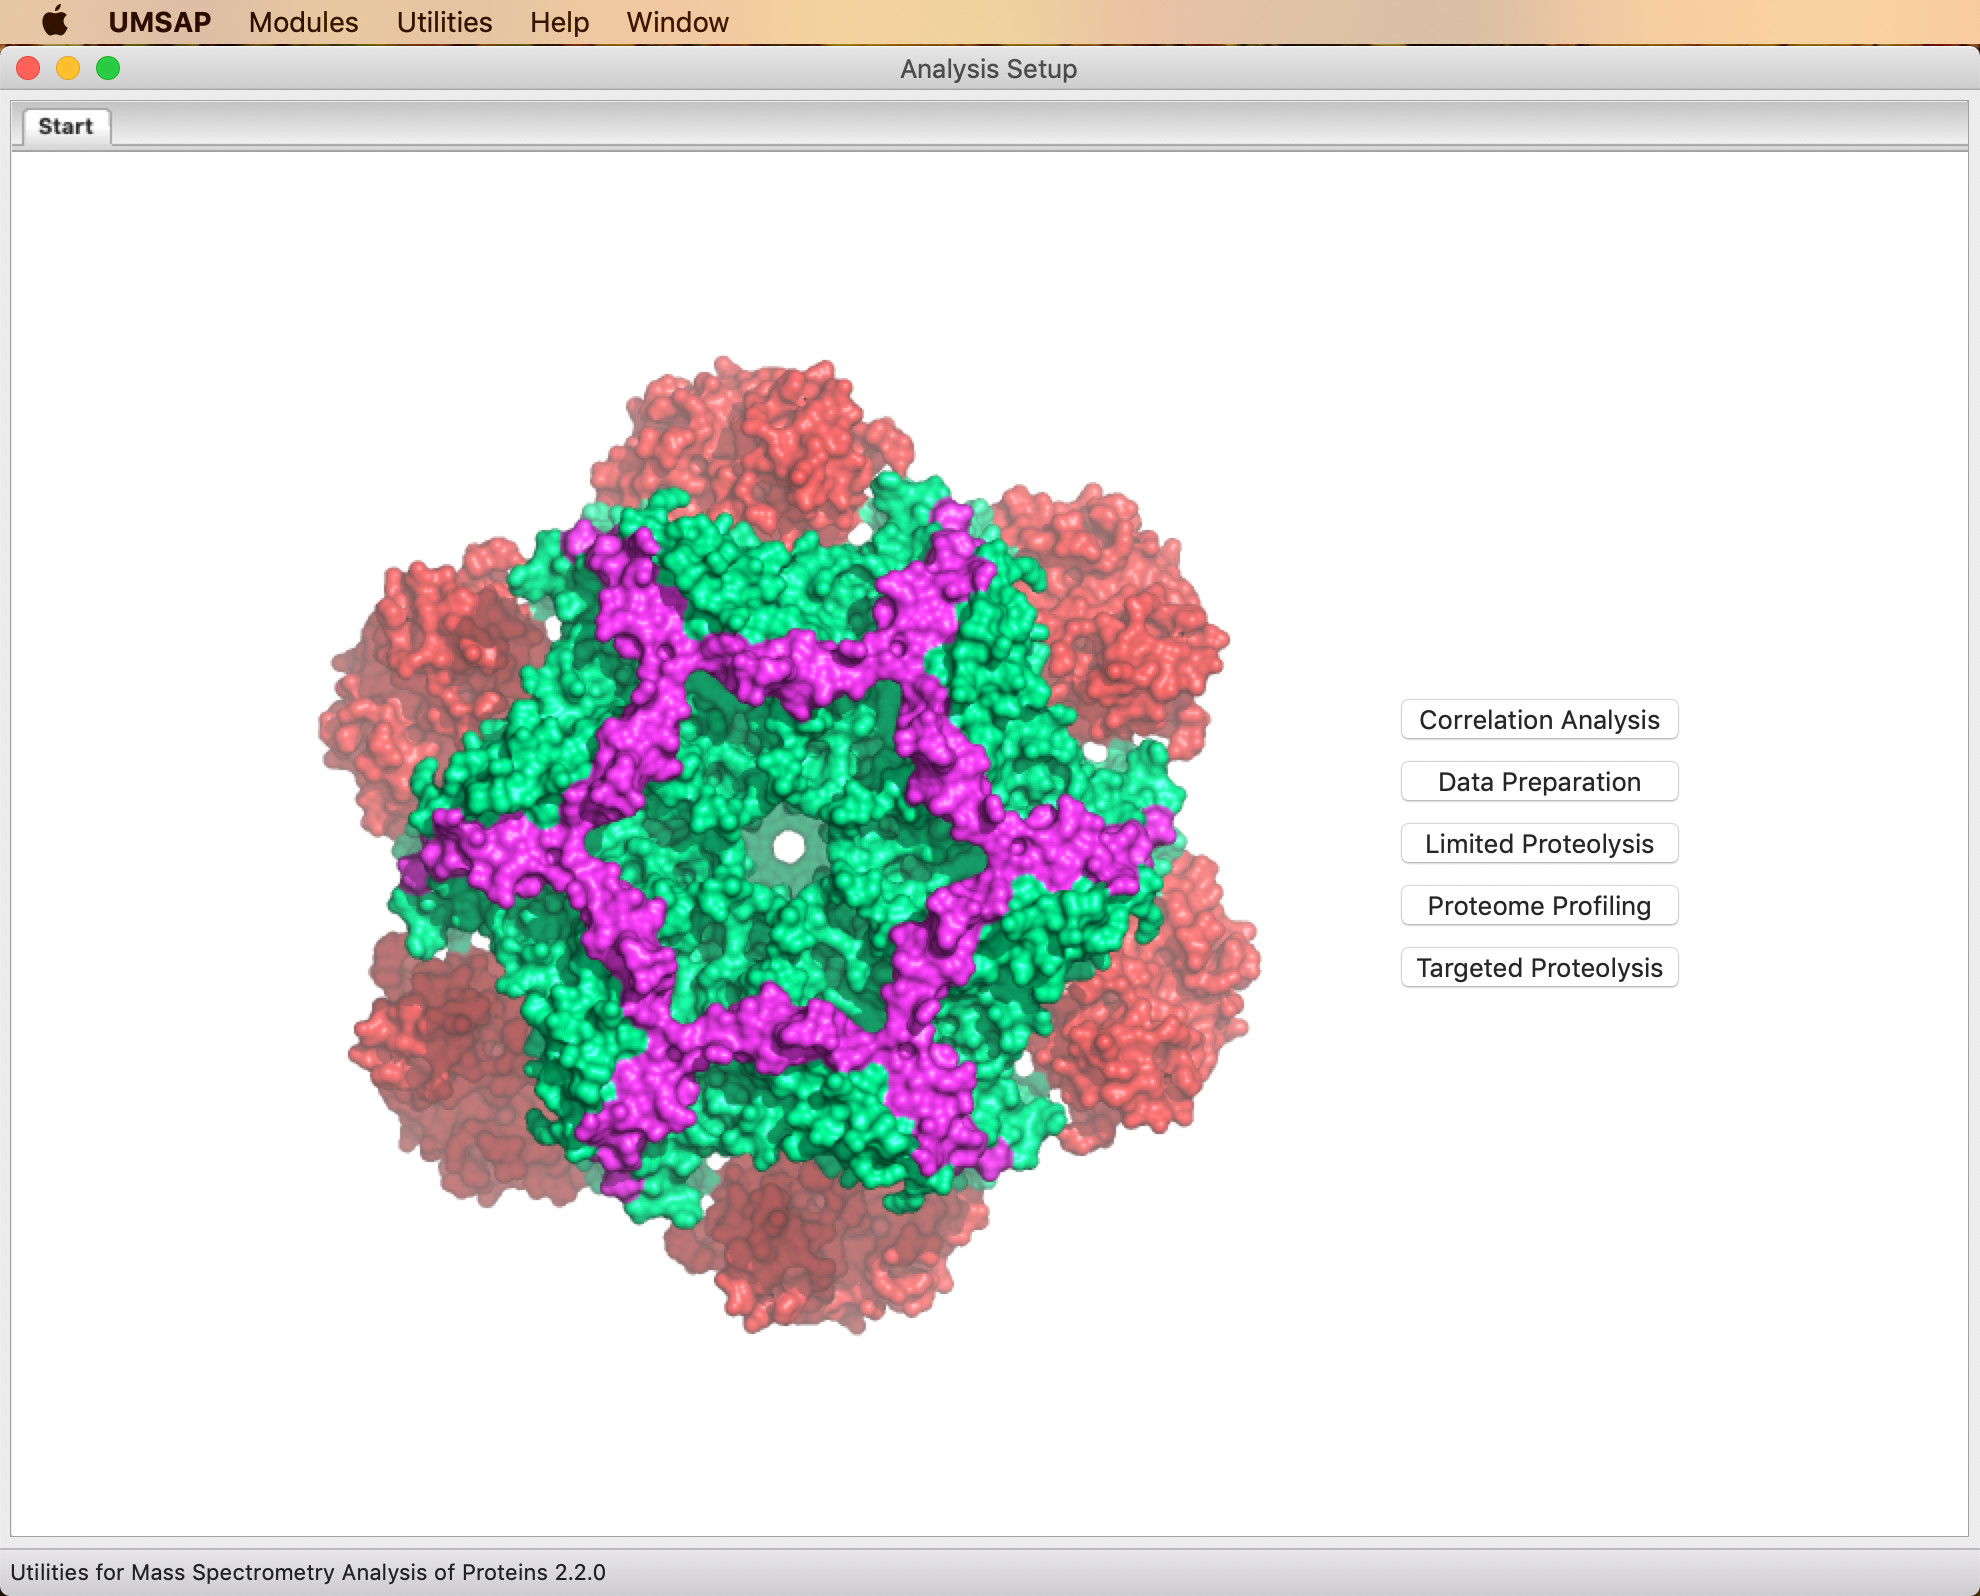
\includegraphics[width=0.7\textwidth]{./IMAGES/MAIN-WINDOW/mainwindow.jpg}
    \caption[The main window of UMSAP]{\textbf{The main window of UMSAP.} From
this window users can access all the available Modules and Utilities.} 
    \label{fig:mainWindow}
    \vspace{-5pt}
\end{figure}  

\section{The input files}
\label{sec:dataFile}

UMSAP has two main input files. One file contains the detected peptide sequences
after all peak assignments have been completed, and the other file contains the
detected proteins. The program expects these files to be plain text files containing
a table with the data. Columns in the files are expected to be tab separated. The
first row in the files is expected to contain only the names of the columns. There
is no limit in the amount and type of data present in the Data files. However, each
module will expect certain columns to be present. Columns not needed by the modules
will be ignored.

In addition, certain modules use other input files as well. The modules Limited Proteolysis
and Targeted Proteolysis use fasta files containing the sequences of
the recombinant and native proteins used in the experiments. The first sequence
found in the fasta file is assumed to be the sequence of the recombinant protein.
The second sequence found in the fasta file is assumed to be the sequence of the
native protein. All other sequences found in the fasta file are discarded. If the
sequence of the native protein is given UMSAP performs a sequence alignment between
the native and recombinant sequences. The alignment allows UMSAP to translate the
results obtained with the residue numbers of the recombinant protein to the residue
numbers of the native protein. This is done to facilitate future comparison of results
between different recombinant proteins of the same native protein. However, when
analyzing the results of the alignment UMSAP assumes that the recombinant and native
sequences differs only in the N and C-terminal tags while the sequence between the
tags is identical. If this is not the case, e.g. there are point mutations or
insertion/deletion in the sequence of the recombinant protein no native sequence
should be given to UMSAP.

\section{The output files}
\label{sec:outFile}

Results generated by UMSAP will be saved in two folders and a file with extension
umsap (\autoref{fig:outFolder}). Direct manipulation of the umsap file and files
within these folders should be avoided. UMSAP provides a way to manage them through
the UMSAP Ctrl window (\autoref{chap:umsapCtrl}). Nevertheless, all the files created
by UMSAP are plain text files with JSON or CSV (tab separated) format, in order for
users to be able to read their content. Changing the content of the files is highly
discouraged as this will lead to errors in the reliability and visualization of the
results obtained with UMSAP.

The folder Input{\_}Data{\_}Files contains a copy of the input files used for the analysis
in the project. When adding a new analysis to the project, the new input files used
will be copied to the Input{\_}Data{\_}Files folder. The date and time of the analysis will
be added to the name of the files to avoid overwriting existing files inside the folder.

The folder Steps{\_}Data{\_}Files contains a folder for each analysis in the project.
These folders contain the main results for the analysis as well as a step by step
account of the calculations and any further analysis performed after the main results
were created.

The umsap file contains information about all the analysis in the project and allows
managing the project and the visualization of the results. An unlimited number of
analysis can be added to any given umsap file. UMSAP will never overwrite or replace
an umsap file, instead new analysis will be added to the selected umsap file.

\begin{figure}[h]
    \centering
    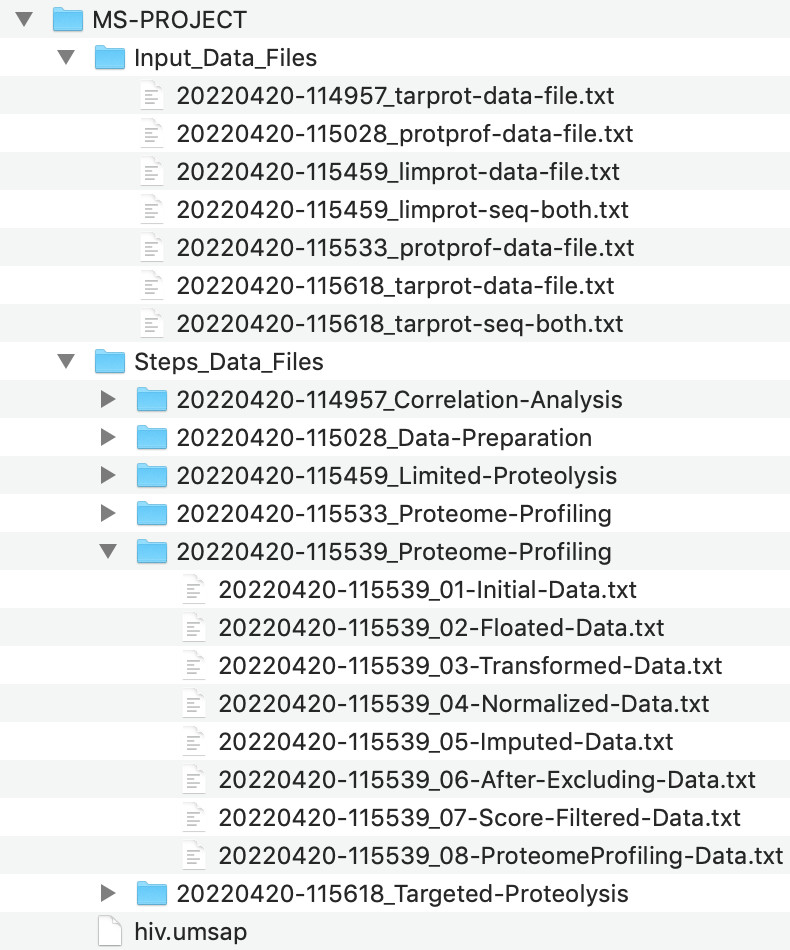
\includegraphics[width=0.7\textwidth]{./IMAGES/OUTPUT/folder.jpg}
    \caption[Structure of the output generated by UMSAP]{\textbf{Structure of the
output generated by UMSAP.} Results are saved in the Steps{\_}Data{\_}Files folder. The
umsap file allows managing and visualizing the results.} 
    \label{fig:outFolder}
    \vspace{-5pt}
\end{figure}

\section{Using Utilities for Mass Spectrometry Analysis of Proteins}

Once the input files are ready to be analyzed, using UMSAP is straightforward. Just
open the program and select a module or utility. In the new tab created in the Analysis
Setup window (\autoref{fig:mainWindow}), fill in the needed
information and hit the Start Analysis button at the bottom of the tab. Depending on
the amount of data and the complexity of the analysis to perform it may take a few
minutes for the program to complete the task at hand. While the analysis is running, a
window, containing a progress bar, will appear. This window will give a rough guess
of the remaining time needed to complete the current analysis and will report any error
encountered. In the case of encountering an unexpected error, it will be helpful if
users send a crash report to umsap@umsap.nl, so we can correct them. 

In order to make the program as user-friendly as possible help messages will pop up
from buttons and labels. The help messages will contain a brief description of what
is the button or label for and what input is expected from the user. In this way, users
can find basic information about a particular element of the interface without needing
to go to the manual or online tutorials. If more information is needed, users may
consult the manual or click the Help button at the bottom of the module/utility tab to
read an online tutorial. 

Depending on the module or utility just run, new windows will be created to show a
graphical representation of the results. All plots support to zoom into a rectangular
selection of the plot and to reset the zoom level.

\section{Navigating through Utilities for Mass Spectrometry Analysis of Proteins}

The entries Modules and Utilities will be available in the menu of every window.
The entry Modules in the menu gives direct access to all modules. The same is true for
the Utilities entry. These menu entries are the fastest way to access all the functions
in UMSAP. In a typical UMSAP session, users will work with different independent windows
simultaneously. The windows have descriptive names, so users can quickly guess the content
of any window. The scheme of the windows name is
\textit{File Name - Utilities or Module Name - ID of the Analysis}. For example, the window
with name \textit{hiv.umsap - Target Proteolysis - 20220420-115618 - Cleavage Sites} will be
displaying the Targeted Proteolysis analysis with ID \textit{20220420-115618 - Cleavage Sites} from
file hiv.umsap.

A list of current shortcuts is given in \autoref{table:shortcuts}.

\begin{table}[h!]
    \centering
    \begin{tabular}{l l l}
        \hline
        \multicolumn{1}{c}{Shortcut} & \multicolumn{1}{c}{Action}& \multicolumn{1}{c}{Window}\\
        \hline
        Alt+Cmd+L  &Create the Limited Proteolysis tab &All\\
        Alt+Cmd+P  &Create the Proteome Profiling tab  &All\\
        Alt+Cmd+T  &Create the Targeted Proteolysis tab&All\\
        Cmd+R      &Read umsap file                    &All\\
        Cmd+A      &Show all peptides                  &Limited Proteolysis\\
        Cmd+L      &Toggle Band/Lane selection mode    &Limited Proteolysis\\
        Cmd+S      &Export sequence alignments         &Limited Proteolysis\\
        Alt+Shift+I&Export all images                  &Multiple plots\\
        Alt+Shift+Z&Reset all zooms                    &Multiple plots\\
        Shift+I    &Export main plot image             &Multiple plots\\
        Shift+Z    &Reset main plot zoom               &Multiple plots\\
        Alt+I      &Export secondary plot image        &Multiple plots\\
        Alt+Z      &Reset secondary plot zoom          &Multiple plots\\
        Shift+A    &Add label to Volcano plot          &Proteome Profiling\\
        Shift+P    &Toggle Pick label / Select protein &Proteome Profiling\\
        Shift+Cmd+A&Apply all Filters                  &Proteome Profiling\\
        Shift+Cmd+F&Auto apply all Filters             &Proteome Profiling\\
        Shift+Cmd+R&Remove selected Filters            &Proteome Profiling\\
        Shift+Cmd+Z&Remove last applied Filter         &Proteome Profiling\\
        Shift+Cmd+X&Remove all Filters                 &Proteome Profiling\\
        Shift+Cmd+C&Copy Filters                       &Proteome Profiling\\
        Shift+Cmd+V&Paste Filters                      &Proteome Profiling\\
        Shift+Cmd+S&Save Filters                       &Proteome Profiling\\
        Shift+Cmd+L&Load Filters                       &Proteome Profiling\\
        Shift+Cmd+E&Export filtered data               &Proteome Profiling\\
        Cmd+P      &Show Data Preparation results      &Results plot\\
        Cmd+D      &Duplicate result window            &Results plot\\
        Cmd+E      &Export data                        &Results plot\\
        Cmd+I      &Export image                       &Results plot\\
        Cmd+K      &Clear all selections               &Results plot\\
        Cmd+Z      &Reset the zoom       on a plot     &Selected plot\\
        Cmd+S      &Export sequence alignments         &Targeted Proteolysis\\
        Cmd+C      &Copy                               &Text and Tables\\
        Cmd+X      &Cut                                &Text and Tables\\
        Cmd+V      &Paste                              &Text and Tables\\
        Cmd+A      &Select all                         &Text and Tables\\
        Cmd+A      &Add analysis                       &UMSAP Ctrl\\
        Cmd+X      &Delete analysis                    &UMSAP Ctrl\\
        Cmd+E      &Export analysis                    &UMSAP Ctrl\\
        Cmd+U      &Reload file                        &UMSAP Ctrl\\
        \hline		
    \end{tabular}
    \caption[List of built-in keyboard shortcuts]{\textbf{List of built-in keyboard
    shortcuts.} Windows users should replace Cmd with Ctrl.}
    \label{table:shortcuts}
\end{table}

\section{Backward compatibility}
\label{sec:backwardCompatibility}

Unfortunately, UMSAP 2.2.0 is not capable to read any file generated with previous
versions of UMSAP.